% !TEX program = xelatex
% !BIB program = biber

\documentclass[11pt]{article}

\usepackage{biblatex}
\usepackage{listings}
\usepackage{xcolor}
\usepackage{fontspec}
\usepackage{graphicx}
\usepackage{amsmath}
\usepackage{amssymb}
\usepackage{float}
\usepackage{arydshln}

\setmonofont[
  Contextuals={Alternate},
  Scale=0.8
]{Fira Code}

\addbibresource{viper.bib}
\addbibresource{silicon.bib}
\addbibresource{patterns.bib}
\addbibresource{intellij.bib}
\addbibresource{caffeine.bib}


\parskip=1em
\parindent=0pt

\definecolor{codegrey}{rgb}{0.9,0.9,0.9}
\definecolor{commentgrey}{rgb}{0.5,0.5,0.5}

\lstdefinestyle{mystyle}{
    basicstyle=\ttfamily,
    keywordstyle=\bfseries,
    commentstyle=\color{commentgrey},
    %backgroundcolor=\color{codegrey},
    frame=single,
    numbers=left,
}
\lstset{style=mystyle}

\DeclareMathOperator{\perm}{\mathbin{\#}}

\begin{document}

    \pagenumbering{gobble}
    \begin{titlepage}
        \begin{center}
            \textit{Bachelor's Thesis}\\
            \vspace{0.5cm}
            \textbf{\Huge Performance Improvements on a Program Verifier}\\
            \vfill   
            Fabian Bösiger\\
            Supervised by Dr. Malte Schwerhoff\\
            \vspace{0.2cm}
            Programming Methodology Group\\
            Department of Computer Science\\
            ETH Zürich\\
            \vspace{0.2cm}
            \today
        \end{center}
    \end{titlepage}
    \newpage

    \begin{abstract}
        \parskip=1em
        \parindent=0pt
        \noindent

        This thesis explores ways to improve performance of
        the Silicon program verification backend is for the Viper
        verification infrastructure.
        
        In a first Part,
        we explore the concept of applying the flyweight pattern on AST terms.
        Applying the flyweight pattern avoids multiple instances of structurally equal terms
        existing at the same time. This allows us to replace structural and recursive
        equality checks with reference equality checks, with the goal of improving performance of equality checks.

        In a second Part, we introduce more sophisticated ways to join back together symbolic execution paths in
        Silicon after branching on conditional expressions, implications and if-statements.
    \end{abstract}
    \newpage

    \renewcommand{\abstractname}{Acknowledgements}
    \begin{abstract}
        \parskip=1em
        \parindent=0pt
        \noindent

        I would like to thank my supervisor, Malte Schwerhoff, who provided
        me with the opportunity to write this thesis. The time
        and effort he expended to help and advice me was highly appreciated.

        Thanks to Peter Müller and his Group for sparking interest and providing insight
        into topics such as these.

        Furthermore, I'd like to express my gratitude towards my family for providing
        me with a very pleasant home office environment.
    \end{abstract}
    \newpage

    \tableofcontents
    \newpage

    \pagenumbering{arabic}

    \section{Introduction}

    Viper \cite{viper} is a verification infrastructure on top of which verification tools
    for different programming languages can be built. Silicon \cite{silicon} is a backend for Viper,
    which is based on symbolic execution. To advance program verification in practice,
    fast verification is crucial as it provides a more streamlined experience for developers.
    This is the reason why one of Silicon's stated goals is performance:

    \begin{quote} 
        ``The verifier should enable an IDE-like experience: it should be
        sufficiently fast such that users can continuously work on verifying
        programs [...]'' \cite{silicon}
    \end{quote}

    In this thesis, we explore two different approaches to improving performance of Silicon.

    Silicon internally uses abstract syntax trees (AST) to represent
    the structure of a program as a tree data structure. As with any other tree structure,
    AST's can be traversed, searched, transformed and so forth. During such operations,
    subtrees within the AST are potentially checked for equality many times.  Moreover, equality checks
    also occur in operations on collections of AST subtrees, for example in finding
    a specific subtree, which may add additional performance overhead.

    Equality checks can't easily be avoided, but they can be implemented in a more performant way.
    Currently in Silicon, new term instances are created independently of already existing ones, which potentially leads 
    to the coexistence of multiple structurally equal term instances. Subterm equality is checked in a
    structural and recursive manner. In a first Part of working towards a potential improvement in performance,
    we explore the concept of applying the flyweight pattern \cite{patterns} on AST terms to only ever have
    one instance of some term structure, thus avoiding the need for structural and recursive equality checks.

    When verifying a program, Silicon uses the symbolic execution approach, where the program is interpreted,
    and a symbolic state keeps track of all possible program states at the current point of execution, for all
    possible input values of the program. When encountering certain expressions or statements, for example an
    if-statement, symbolic execution branches with the assumptions of the corresponding program path.

    Silicon currently only joins these branches back together for some simple cases. In other cases,
    branches aren't joined back together, which results in all statements later down the verification path
    being evaluated essentially twice, but with different assumptions in each branch. Both of these
    verification paths may branch again, potentially leading to exponential growth in active branches.
    In an effort to improve performance, the second part of this thesis focuses on implementing more
    joins for execution paths, which ultimately leads to fewer active branches.

    \part{Flyweight AST's;\newline A Study in Applied Laziness}
    \begin{center}
        \vspace{3cm}
        
\includegraphics[width=0.7\textwidth]{fly}
    \end{center}

    \newpage
    \section{Approach}

    \subsection{Implementation of Flyweight AST's}
    
    The AST used in Silicon is immutable, so the flyweight pattern \cite{patterns}
    can be applied on AST terms.
    To do this, a pool of term instances is maintained. Whenever a term
    is to be created, the components of this new term is compared with the
    pool of existing terms. If a term with the same components already exists,
    a reference to the existing term is returned and
    the creation of a new instance is avoided. Otherwise, a new term is created and added to
    the pool.

    This gives the guarantee that there are no two instances of the
    same term in our pool, meaning every two structurally equal terms point to the same
    underlying object in memory. Comparing terms for structural equality then boils
    down to a cheap reference equality check, and recursive equality checks can be avoided.

    \subsection{Automate Boilerplate Generation using Macros} \label{boilerplate-generation-using-macros}

    Silicon's AST representation of the Viper language consists of nearly 100 different terms,
    all with boilerplate implementations for different operations.
    Our changes introduce additional boilerplate code to each term.

    Our AST's shouldn't only be flyweight in the sense of the implementation pattern, but also
    regarding development time and effort. This is why we want to avoid such boilerplate
    code and instead automatically generate it using Scala's support for macro annotations.
    Additional benefits of using macro annotations include improvements in code
    readability and maintainability. Experimenting with code changes will become a matter
    of editing a single macro instead of editing each term individually.
    Terms which may be added in the future are easier to implement.

    \newpage
    \section{Implementation}

    \subsection{Implementation of the Flyweight Pattern} \label{implementation-flyweight-pattern}

    The implementation of the flyweight pattern works as follows:

    \begin{enumerate}
        \item The constructor of a term is made private so that new term instances can't be created via
            the \texttt{new} keyword, but only via the \texttt{apply} method.
        \item For every term, we create a map which maps the fields of the term to the term itself.
            This allows us to later look up whether a structurally equal term already was created.
        \item In the \texttt{apply} method, we check the pool for structurally equal instances,
            and if one exists, we return it instead and thus avoid creating a new instance of the
            same term.
        \item If no structurally equal instance exist, we create a new instance via the \texttt{new}
            keyword, add it to the pool and return it.
    \end{enumerate}

    As an example, the implementation of the flyweight pattern for the \texttt{Plus} term is shown here:

    \begin{lstlisting}[language=Scala, caption={Implementation of the flyweight pattern.}, label={lst:flyweight-pattern}]
        class Plus private (val p0: Term, val p1: Term) {
            // ...
        }
        
        object Plus extends ((Term, Term) => Term) {
            // Maps fields of the term to the term instance itself.
            var pool = new TrieMap[(Term, Term), Term]
        
            def apply(e0: Term, e1: Term): Term = {
                pool.get((e0, e1)) match {
                    // If no structurally equal term exists,
                    // create a new one.
                    case None => 
                        val term = new Plus(e0, e1)
                        pool.addOne((e0, e1), term)
                        term
                    // If a structurally equal term exists,
                    // return a reference to it instead.
                    case Some(term) => 
                        term
                }
            }

            // ...
        }       
    \end{lstlisting}

    \subsection{A Macro Annotation for Code Generation}

    The code for the flyweight macro annotation exists as a subproject within Silicon. Each term can be
    annotated with \texttt{@flyweight}, which invokes the macro at compile time and 
    rewrites the term in the following way:

    \begin{enumerate}
        \item If an \texttt{apply} method is already defined, rename it to \texttt{\_apply}.
            The already defined apply method can't be discarded because it potentially
            performs AST simplifications.
        \item Define a new \texttt{apply} method which introduces the flyweight pattern
            as discussed in section \ref{implementation-flyweight-pattern}.
            If a new instance has to be created, either use  the previously 
            defined \texttt{\_apply} method
            if it exists, else simply create an instance using the \texttt{new} keyword.
        \item Generate an \texttt{unapply} method.
        \item Generate a \texttt{copy} method that calls \texttt{apply} instead of creating
            instances via \texttt{new} such that the flyweight pattern can't be bypassed
            when copying a term.
        \item Override \texttt{hashCode} to use \texttt{System.identityHashCode}.
    \end{enumerate}

    This process of rewriting terms can be nicely illustrated in an example
    which considers the program input and output of our macro:

    \begin{lstlisting}[language=Scala, caption={Input code given to the macro.}, label={lst:macro-input}]
@flyweight
class Plus(val p0: Term, val p1: Term)
    extends ArithmeticTerm with BinaryOp[Term]
{
    override val op = "+"
}

object Plus extends ((Term, Term) => Term) {
    import predef.Zero

    def apply(e0: Term, e1: Term): Term = (e0, e1) match {
        case (t0, Zero) => t0
        case (Zero, t1) => t1
        case (IntLiteral(n0), IntLiteral(n1)) => IntLiteral(n0 + n1)
        case _ => new Plus(e0, e1)
    }
}        
    \end{lstlisting}

    \begin{lstlisting}[language=Scala, caption={Output code generated by our macro.}, label={lst:macro-output}]
class Plus private[terms] (val p0: Term, val p1: Term)
    // Superclasses and implemented traits are preserved from input.
    extends ArithmeticTerm with BinaryOp[Term]
{
    // Override hashCode.
    override lazy val hashCode = System.identityHashCode(this)

    // Generate copy method which uses the generated apply method.
    def copy(p0: Term = p0, p1: Term = p1) = Plus(p0, p1)

    // Preserved from input.
    override val op = "+"
}

object Plus extends ((Term, Term) => Term) {
    import scala.collection.concurrent.TrieMap
    var pool = new TrieMap[(Term, Term), $returnType]

    // Define new apply method which uses the flyweight pattern.
    def apply(e0: Term, e1: Term): Term = {
        pool.get((e0, e1)) match {
            case None => 
                val term = Plus._apply(e0, e1)
                pool.addOne((e0, e1), term)
                term
            case Some(term) => 
                term
        }
    }

    // Generate unapply method.
    def unapply(t: Plus) =
        Some((t.p0, t.p1))

    // Preserved from input.
    import predef.Zero

    // Rename existing apply method to _apply.
    // AST simplifications implemented are thus preserved.
    def _apply(e0: Term, e1: Term): Term = (e0, e1) match {
        case (t0, Zero) => t0
        case (Zero, t1) => t1
        case (IntLiteral(n0), IntLiteral(n1)) => IntLiteral(n0 + n1)
        case _ => new Plus(e0, e1)
    }
}       
    \end{lstlisting}

    %\subsubsection{Classes or Case Classes}

    %\subsubsection{Macro Annotations on Nodes}

    %\subsubsection{Clear Pools after each File}

    %\subsubsection{AST Reduction for Builtin Equals}

    %\subsubsection{Equality Defining Members}

    %\subsection{IntelliJ Support}

    \subsection{Flyweight Macro Support for IntelliJ}

    The Viper infrastructure is written in the Scala programming language.
    Scala has support for metaprogramming using macros, which provide
    a nice and easy way for metaprogramming and
    are regularly used. For a nice programming experience
    using macros, IDE support should ideally be provided. In this case, we use the IntelliJ IDE.
    However, Scala macros are not supported natively by the IntelliJ IDE, 
    as it is difficult for IDE's to provide proper syntax highlighting.:

    \begin{quote}
        ``Since IntelliJ IDEA’s coding assistance is based on static code analysis,
        the IDE is not aware of AST changes, and can’t provide appropriate code
        completion and inspections for the generated code.'' \cite{intellij}
    \end{quote}

    In the example of our flyweight macro, IntelliJ is not aware that
    the method \texttt{apply} is generated, and thus reports an error
    wherever a term is applied. To fix this issue for the IntelliJ IDE,
    we provide a plugin which
    can be easily installed in IntelliJ, and fixes the highlighting
    issues for the flyweight macro.

    \subsubsection{Towards Full Scala Macro Support for IntelliJ} \label{full-scala-macro-support}

    The plugin discussed is hard coded to only support the flyweight macro.
    To encourage more experimentation using macros, it is of advantage
    to have a plugin which supports macros that may be modified, for example
    by generating additional methods.

    To support this kind of more dynamic plugin, the macro is modified to
    dump all generated method signatures into a configuration file.
    This configuration file is then read by the IntelliJ plugin,
    which now knows the signatures of the methods generated by the macro.
    Whenever the macro is modified and the program is compiled again,
    the configuration file is rewritten, and the IntelliJ plugin is
    aware of the changes.

    \newpage
    \section{Evaluation}


    \subsection{Performance of Different Data Structures}
    
    % \begin{center}
    %     \begin{tabular}{ |l|c|c| } 
    %     \hline
    %     Resources Used & VerCors \\ 
    %     \hline
    %     Number of Parallel Verifiers & 1 \\
    %     \hline
    %     Repetitions & 10 \\ 
    %     \hline
    %     \end{tabular}
    % \end{center}

    The table below shows the relative performance change of the flyweight implementation
    using different map data structures for the pool implementation which stores
    term instances.

    \begin{center}
        \begin{tabular}{ ll } 
        \hline
        Data Structure & Relative Performance Change \\ 
        & (Negative is better) \\
        \hline
        \texttt{mutable.HashMap} & -1.3\% \\ 
        \texttt{mutable.WeakHashMap} & -0.2\% \\
        \texttt{concurrent.TrieMap} & -0.2\% \\
        \texttt{concurrent.ListMap} & +89.5\% \\ 
        \hline
        \end{tabular}
    \end{center}

    Dedicated maps for caching such as Caffeine \cite{caffeine} where tested as well,
    but they add no advantage over maps
    implemented in the Scala standard library, performance- or otherwise.
    Not that the pool used in the flyweight pattern is
    not used like a classical caching system. Eviction policies for example
    are unnecessary as terms are required to stay in the pool at least as long
    as other references to the term still exist. 

    As expected, the use of \texttt{ListMap} significantly worsens performance,
    as linear time with respect to existing terms is required for a lookup operation.
    The performance of \texttt{HashMap}, \texttt{WeakHashMap}, \texttt{TrieMap}
    are very similar to the base implementation in this benchmark.
    As Silicon may use multiple verifier instances in parallel,
    we chose \texttt{TrieMap} for the concluding performance evaluation, as it has
    the additional benefit of being concurrency-safe.
    

    \subsection{Concluding Performance Evaluation}

    To measure the performance difference, programs generated by the VerCors,
    Prusti, Gobra and Vyper frontends are considered. The number of parallel 
    verifiers is set to one, however as Scala's \texttt{mutable.TrieMap} is used,
    the flyweight pattern would still work in a parallelized environment. The benchmarks is repeated ten times, where the
    slowest and fastest verification time are ignored. The flyweight implementation on average 2\% was slower,
    which is still within the standard derivation of 2.9\%.

    %\subsection{Memory Consumption}

    %\subsection{Memory Pool Hit Rate}

    %\subsection{AST Node Count on Equality Checks}

    \subsection{Why did Flyweight Fail}

    Although reference equality checks are certainly much faster than recursive structural equality
    checks, changing terms to use the Flyweight pattern didn't result in measurable performance improvements.

    There are some reasons why this might be the case. First, there may be not enough structurally
    equal term instances to justify
    a flyweight pattern. To explore this possibility, we measured the hit percentage
    of looking up terms in the flyweight pool. Many structurally different term instances would lead to
    a low hit percentage, which would render a flyweight pattern inefficient. In our
    benchmarks, a hit percentage of around 83\% was measured, meaning that on average,
    for every term created and added to the flyweight pool, four structurally equal terms could be avoided.

    Another reason may lie in the depth of the term on an equality check. If
    the terms are very flat when checking for equality, the additional performance overhead of structural, recursive equality checks becomes negligible compared to reference equality checks, even
    if many equality checks take place. To support this hypothesis, we counted the number of subterms
    contained term at every equality check. For example, if \texttt{Plus(1, Minus(2, 3))} was checked for equality,
    we count 5 contained subterms, once \texttt{Plus}, once \texttt{Minus} and three integer literals.
    Figure \ref{fig:node-count} shows the average subterm count for each term. On average,
    a term contains around 14 subterms on equality check.

    \begin{figure}[H]
        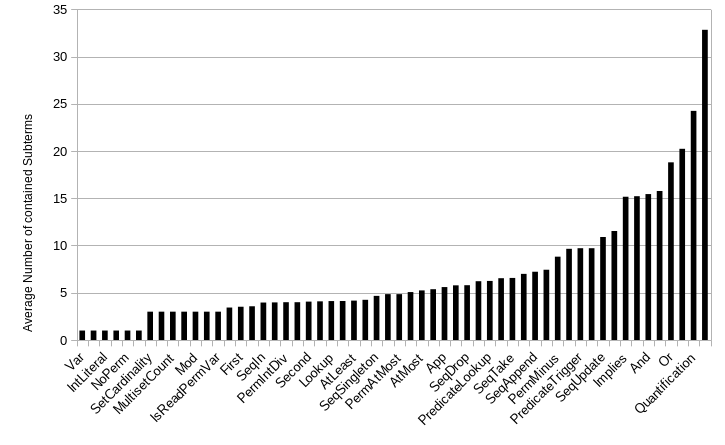
\includegraphics[width=\linewidth]{node-count.png}
        \caption{Number of subterms contained in a term on equality check.}
        \label{fig:node-count}
    \end{figure}

    To summarize, avoiding on average four structurally equal term instances which contain
    on average 14 subterms is most likely not enough to justify the overhead introduced by the flyweight pattern.


    %\subsection{Automatic Code Generation}

    \subsection{An Example of Experimenting with Macros}

    Although the flyweight pattern itself didn't have a significant impact on performance,
    the macro annotation developed to implement the flyweight pattern can
    be quickly modified to perform experiments or benchmarks on the Silicon AST.

    In the following example, the macro is edited to ignore AST simplifications.
    To achieve this, we avoid calling \texttt{\_apply}, which performs AST simplifications.
    Instead, we directly create instances using the \texttt{new} keyword.
    Using the macro, this can be done quickly for all terms by only modifying three lines
    instead of rewriting every term manually.

    \begin{lstlisting}[language=Scala, caption=Use AST simplifications as normal.]
def apply(..$fields) = {
    // ...
    ${
        if (hasRenamedApplyMethod)
            // AST simplifications are potentially performed when
            // creating instances via _apply.
            q"${termName}._apply(..${fieldNames})"
        else
            q"new $className(..${fieldNames})"
    }
    // ...
}  
    \end{lstlisting}

    \begin{lstlisting}[language=Scala, caption=Modified macro to ignore AST simplifications.]
def apply(..$fields) = {
    // ...
    ${
        q"new $className(..${fieldNames})"
    }
    // ...
}  
    \end{lstlisting}


    \newpage
    \section{Future Work}

    \begin{itemize}
        \item For the current state of Silicon and the Viper Language,
            there is little potential left to be explored in the direction
            of flyweight AST's. Nevertheless, if the structure of Silicon's AST's
            changes in the future, maybe if the structure of the intermediate verification
            language changes to a more functional style, AST's may become larger and
            flyweight AST's provide an actual performance improvement.
        \item The macro annotation developed to modify Silicon's Terms
            invites to various experiments. Reducing boilerplate code,
            adding a simpler way to apply AST simplifications are some
            ideas.
        \item In principle, the generic plugin implementation introduced in
            section \ref{full-scala-macro-support} can be used in projects other
            than Silicon which make use of their own macro annotations.
            The plugin is not yet fully fleshed out and can be developed
            further to be faster and provide more support for a
            wider range of macro types. If done right, the further development
            of such a plugin can be a valuable addition to
            development of Scala programs in the IntelliJ IDE.
    \end{itemize}

    \newpage
    \part{Joining;\newline Getting Rid of the Branches}
    \begin{center}
        \vspace{2cm}
        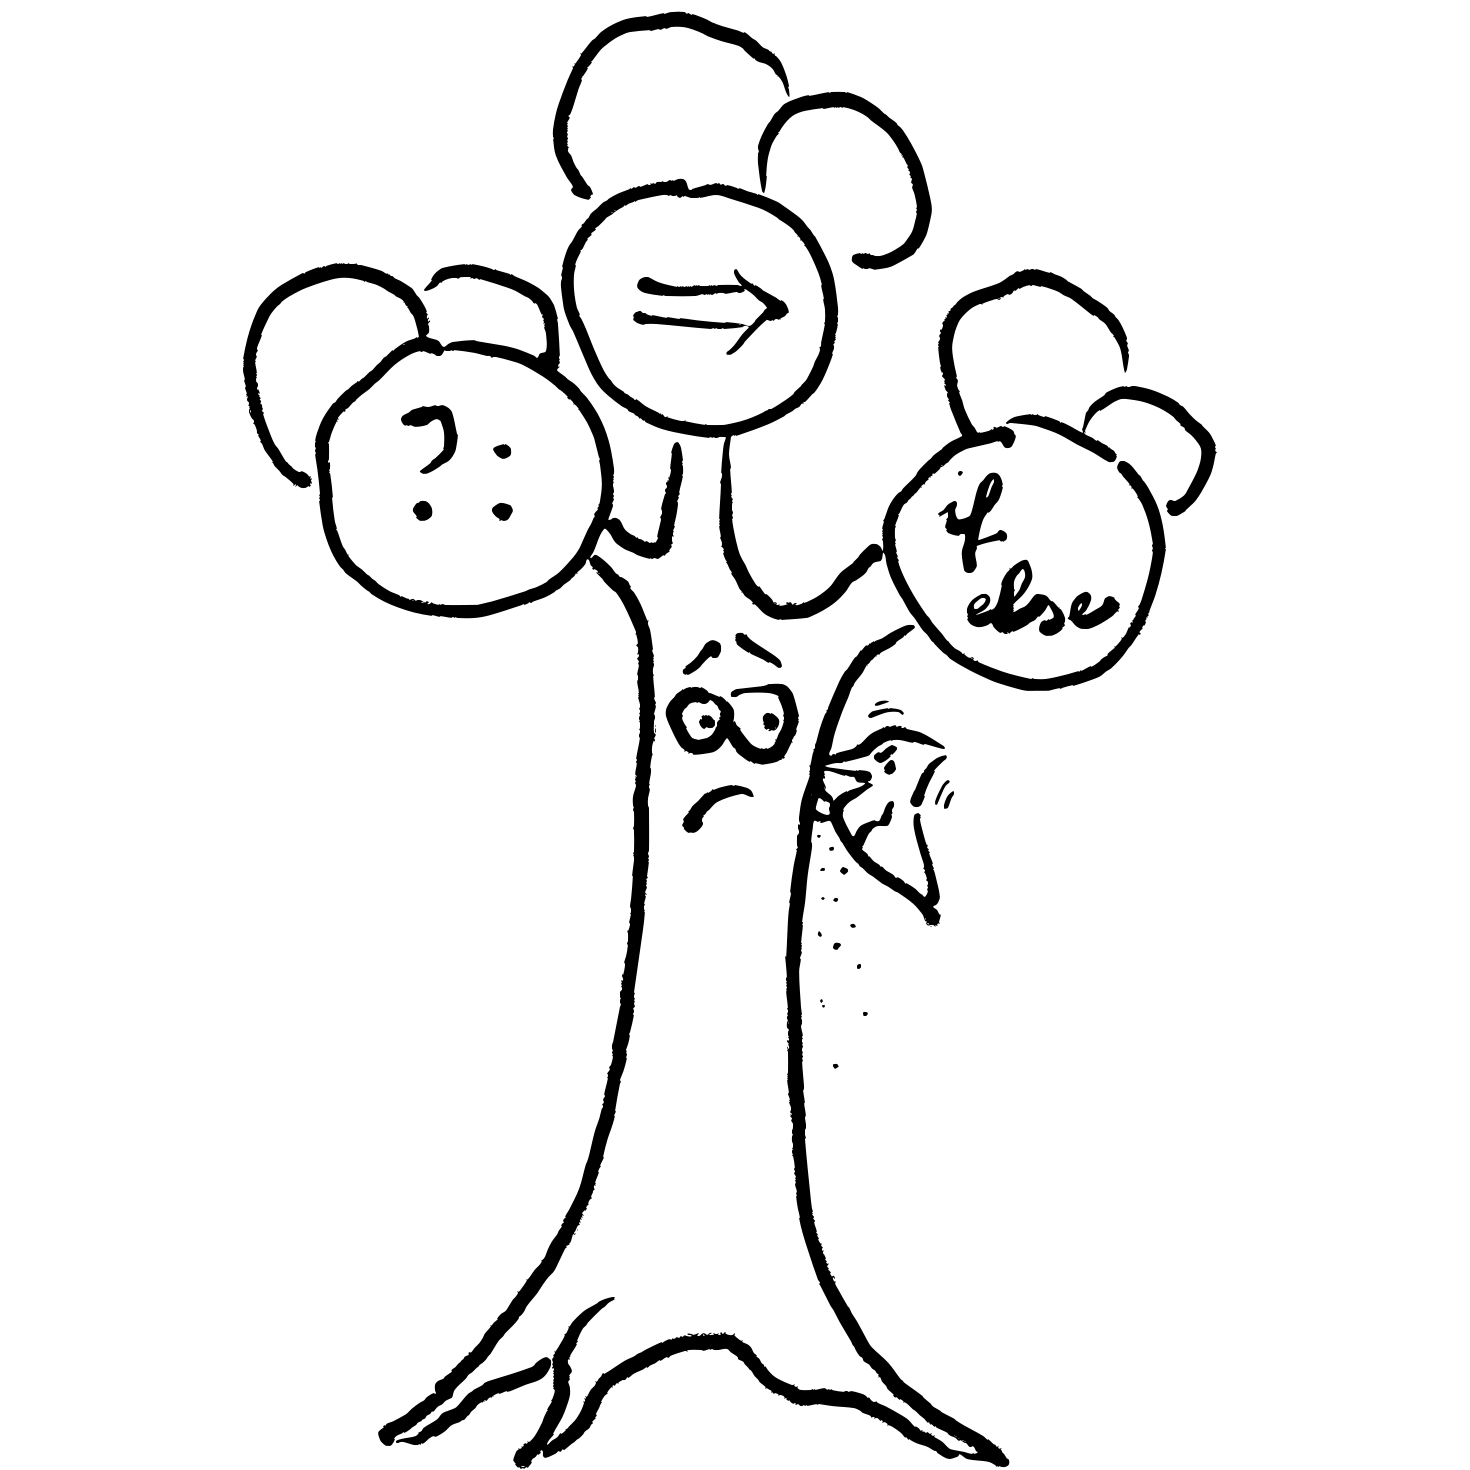
\includegraphics[width=0.9\textwidth]{tree}
    \end{center}

    \newpage
    \section{Approach}

    \subsection{Where to Join}

    \subsubsection{Conditional Expressions}

    Consider a conditional expression of the form $Ite(b, e_1, e_2)$.
    As Silicon evaluates this expression, and $b$ cannot definitely be evaluated to true or false,
    two branches are created, the first one assumes that $b$
    is true, and the second one that $b$ is false, and symbolic execution is continued for both branches.


    \subsubsection{Implications}

    Similar to conditional expressions, symbolic execution branches on implications too. Consider
    an implication of the form $b \implies i$. The first branch assumes that $b$ is true and
    consequently the implication $i$ holds. The second branch assumes that $b$ is false and the
    implication $i$ may or may not hold. 

    \subsubsection{If-Statements} \label{if-statements}

    Viper is parsed into a Control Flow Graph (CFG) consisting of blocks containing
    statements, and edges which connect blocks. Edges can be unconditional or conditional,
    and can potentially form cycles whenever a back edge is connected to a loop head block.
    Symbolic execution branches whenever a block has more than one outgoing edges.

    To join again at the correct location within the CFG after branching,
    the join point for each corresponding branch point has to be identified.
    We introduce a recursive algorithm which maps each branch point to its corresponding join point,
    if it exists:

    \begin{enumerate}
        \item Initialize a queue of blocks to visit and a list of already visited blocks.
            Traverse the CFG in a breath-first way.
        \item \emph{Recursive Case.} If a block has two outgoing edges, it is a branch point.
            Call this procedure recursively, starting from this branch point.
        \item \emph{Base Case.} If a block is visited which already is included in the visited list,
            return this block as it is the join point corresponding to the branch point where this procedure was called.
    \end{enumerate}

    Special attention has to be paid to loops. If our algorithm follows a back edge before finding a join point,
    it may do the recursion again for the same branch point. To avoid this, all already visited loop head blocks
    are remembered for later recursive invocations. Already visited loop head blocks are not followed again.
    Whenever a join point exists for a branch point created via if-statement, we can now join again similar to
    conditional expressions or implications.

    Branches created by both conditional expressions and implications are already being joined if they are pure.
    Branches resulting from impure conditional expressions and implications,
    and from all if-statements however aren't joined again, meaning that
    all statements later down the verification path are evaluated twice. Both of these
    verification paths may branch again, eventually leading to exponential growth in branches.
    These branches are avoided when joining the symbolic execution paths back together.
    However, joining execution paths requires merging the symbolic state, which
    ultimately produces more complex symbolic state entries.

    Intuitively, the same work has to be done with or without joining. The difference is that
    no joining leads
    to many execution paths with simpler symbolic states, and thus more, but less complex
    invocations of the SMT solver. More joining on the other hand leads to
    fewer execution paths but with more complex symbolic states, resulting in fewer,
    but more complex invocations of the SMT solver.


    \subsection{Merging the Symbolic State} \label{merging-the-symbolic-state}
    
    To formalize the merging process, we define
    a symbolic state $\sigma$ of type $\Sigma := (\Gamma, \Pi, H)$. The entries
    defined as follows:

    \begin{itemize}
        \item A store $\gamma$ of type $\Gamma := Var \to V$ maps local variables to their symbolic values.
        \item A path condition stack $\pi$ of type $\Pi$ records all assumptions that have been made in the current verification path.
        \item A symbolic heap $h$ of type $H$ that records which locations are accessible and their respective symbolic values.
    \end{itemize}

    For the following subsections, assume that after the verification branched under the condition $c$ of type $Bool$,
    two symbolic states $\sigma_1 = (\gamma_1, \pi_1, h_1)$ under the branch condition $c = c_1$, and
    $\sigma_2 = (\gamma_2, \pi_2, h_2)$ under the branch condition $\overline{c} = c_2$ are to be merged,
    resulting in the new state $\sigma_3 = (\gamma_3, \pi_3, h_3)$.

    Note that this core idea could be extended to merge more than two states at once. In practice however,
    no more than two states are merged at once.

    \subsubsection{Merging the Store}

    For merging stores $\gamma_1$ and $\gamma_2$, we consider two cases:

    \begin{enumerate}
        \item For some local variable $x$, we have $x \mapsto v_1 \in \gamma_1$ and $x \mapsto v_2 \notin \gamma_2$.
            In this case, we can simply omit $x$ in the new store $\gamma_3$ as we can assume that $x$ won't
            be needed later down the verification path.
        \item For some local variable $x$, we have $x \mapsto v_1 \in \gamma_1$ and $x \mapsto v_2 \in \gamma_2$.
            In this case, we modify the heap chunk such that $x \mapsto Ite(c_1, v_1, v_2) \in \gamma_3$.
    \end{enumerate}

    \subsubsection{Merging the Heap}

    A heap is essentially a collection of heap chunks, where each heap chunk provides information
    about the location's value and the receiver's permission amount to the location.
    As there may be multiple heap chunks making statements about aliased receivers,
    Silicon provides a mechanism to merge them using a mechanism called state consolidation.
    To merge heaps $h_1$ and $h_2$, we perform the following steps:

    \begin{enumerate}
        \item Every non-quantified heap chunk $c$ for which $c \in h_1$ and $c \in h_2$ holds can be carried over to $h_3$
            without modifications.
        \item Non-quantified heap chunks $c := x.f \mapsto t \perm p$ where $c \in h_1$ and $c \notin h_2$ are modified to
            have permissions only if $c_1$ holds: $c' := x.f \mapsto t \perm Ite(c_1, p, 0) \in h_3$
        \item Finally, $h_3$ can be consolidated to avoid multiple aliasing heap chunks.
    \end{enumerate}

    Quantified heap chunks are of the shape $\forall x: c(x) \implies e(x).f \mapsto v(x) \perm p(x)$.
    In practice, they are rewritten to the equivalent form $\forall x: e(x).f \mapsto v(x) \perm p'(x)$,
    where $p'(x)$ is defined as:

    \begin{math}
        p'(x) = \begin{cases}
            p(x) & \text{if } c(x) \text{ is true,} \\
            0 & \text{else}
        \end{cases}
    \end{math}

    Analogously to non-quantified heap chunks, we can simply modify the permission amounts of
    quantified heap chunks to $p''(x) = Ite(c_1, p'(x), 0)$, where the new chunk has the shape
    $\forall x: c(x) \implies e(x).f \mapsto v(x) \perm p''(x)$.

    \subsubsection{Merging the Path Conditions}

    For path conditions, the functionality for merging is already provided.
    This is done by putting the collected path conditions of each branch
    under an implication with the corresponding branch condition.

    \newpage
    \section{Implementation}

    \subsection{Finding Join Points}

    To find join points within the CFG, the algorithm described in \ref{if-statements} is implemented.
    The algorithm produces a mapping from each branch point to the respective join point. The recursive following of
    CFG edges is modified to return as soon as the join point is reached, and the branches are joined again.

    \subsection{Implementing State Merges}

    Store and heap merges are implemented as according to \ref{merging-the-symbolic-state}.
    Silicon's state however consists of some more fields carrying additional data, that have to be merged with caution.
    Caches within the state are emptied instead of merged for simplicity.

    \begin{lstlisting}[language=Scala, caption={An example Viper program.}, label={lst:viper-example}]
method test(b: Bool) {
    var x: Int := 0
    if (b) {
        x := x + 5
    } else {
        x := x + 7
    }
    x := x + 3
    assert x <= 10
}       
    \end{lstlisting}

    \begin{center}
        \begin{tabular}{ l|l|l }
            Operation & Store & Path Conditions \\
            \hline
            \texttt{var x: Int := 0} & & \\
            \hdashline
            \texttt{x := x + 5} & $x \mapsto 0$ & $b$ \\
            \texttt{x := x + 3} & $x \mapsto 5$ & $b$ \\
            \texttt{assert x <= 10} & $x \mapsto 8$ & $b$ \\
            \hdashline
            \texttt{x := x + 7} & $x \mapsto 0$ & $!b$ \\
            \texttt{x := x + 3} & $x \mapsto 7$ & $!b$ \\
            \texttt{assert x <= 10} & $x \mapsto 10$ & $!b$ \\
        \end{tabular}
    \end{center}

    \begin{lstlisting}[language=Scala, caption={An example Viper program.}, label={lst:viper-example}]
EXECUTE 2:8: var x: Int
Store: (b -> b@1@16),
PCs: ()

EXECUTE 2:8: x := 0
Store: (b -> b@1@16, x -> x@2@16),
PCs: ()

EXECUTE 4:10: x := x + 5
Store: (b -> b@1@16, x -> 0),
PCs: (b@1@16)

EVAL 4:19: x + 5
Store: (b -> b@1@16, x -> 0),
PCs: (b@1@16)

EXECUTE 8:6: x := x + 3
Store: (b -> b@1@16, x -> 5),
PCs: (b@1@16)

EVAL 8:15: x + 3
Store: (b -> b@1@16, x -> 5),
PCs: (b@1@16)

EXECUTE 9:11: assert x <= 10
Store: (b -> b@1@16, x -> 8),
PCs: (b@1@16)

CONSUME 9:13: x <= 10
Store: (b -> b@1@16, x -> 8),
PCs: (b@1@16)

EVAL 9:13: x <= 10
Store: (b -> b@1@16, x -> 8),
PCs: (b@1@16)

EVAL 3:10: !b
Store: (b -> b@1@16, x -> 0),
PCs: ()

EXECUTE 6:10: x := x + 7
Store: (b -> b@1@16, x -> 0),
PCs: (!(b@1@16))

EVAL 6:19: x + 7
Store: (b -> b@1@16, x -> 0),
PCs: (!(b@1@16))

EXECUTE 8:6: x := x + 3
Store: (b -> b@1@16, x -> 7),
PCs: (!(b@1@16))

EVAL 8:15: x + 3
Store: (b -> b@1@16, x -> 7),
PCs: (!(b@1@16))

EXECUTE 9:11: assert x <= 10
Store: (b -> b@1@16, x -> 10),
PCs: (!(b@1@16))

CONSUME 9:13: x <= 10
Store: (b -> b@1@16, x -> 10),
    \end{lstlisting}

    \begin{lstlisting}[language=Scala, caption={An example Viper program.}, label={lst:viper-example}]
[info] EXECUTE 2:8: var x: Int
[info] Store: (b -> b@1@16),
[info] Heap: (),
[info] OHs: (old: ()),
[info] PCs: ()
[info] )
[info] EXECUTE 2:8: x := 0
[info] Store: (b -> b@1@16, x -> x@2@16),
[info] Heap: (),
[info] OHs: (old: ()),
[info] PCs: ()
[info] )
[info] EXECUTE 4:10: x := x + 5
[info] Store: (b -> b@1@16, x -> 0),
[info] Heap: (),
[info] OHs: (old: ()),
[info] PCs: (b@1@16)
[info] )
[info] EVAL 4:19: x + 5
[info] Store: (b -> b@1@16, x -> 0),
[info] Heap: (),
[info] OHs: (old: ()),
[info] PCs: (b@1@16)
[info] )
[info] EVAL 3:10: !b
[info] Store: (b -> b@1@16, x -> 0),
[info] Heap: (),
[info] OHs: (old: ()),
[info] PCs: (!(b@1@16))
[info] )
[info] EXECUTE 6:10: x := x + 7
[info] Store: (b -> b@1@16, x -> 0),
[info] Heap: (),
[info] OHs: (old: ()),
[info] PCs: (!(b@1@16))
[info] )
[info] EVAL 6:19: x + 7
[info] Store: (b -> b@1@16, x -> 0),
[info] Heap: (),
[info] OHs: (old: ()),
[info] PCs: (!(b@1@16))
[info] )

JOIN

[info] EXECUTE 8:6: x := x + 3
[info] Store: (b -> b@1@16, x -> (b@1@16 ? 5 : 7)),
[info] Heap: (),
[info] OHs: (old: ()),
[info] PCs: ()
[info] )
[info] EVAL 8:15: x + 3
[info] Store: (b -> b@1@16, x -> (b@1@16 ? 5 : 7)),
[info] Heap: (),
[info] OHs: (old: ()),
[info] PCs: ()
[info] )
[info] EXECUTE 9:11: assert x <= 10
[info] Store: (b -> b@1@16, x -> x@3@16),
[info] Heap: (),
[info] OHs: (old: ()),
[info] PCs: (x@3@16 == (b@1@16 ? 5 : 7) + 3)
[info] )
[info] CONSUME 9:13: x <= 10
[info] Store: (b -> b@1@16, x -> x@3@16),
[info] Heap: (),
[info] OHs: (old: ()),
[info] PCs: (x@3@16 == (b@1@16 ? 5 : 7) + 3)
[info] )
[info] h = ()
[info] EVAL 9:13: x <= 10
[info] Store: (b -> b@1@16, x -> x@3@16),
[info] Heap: (),
[info] OHs: (old: ()),
[info] PCs: (x@3@16 == (b@1@16 ? 5 : 7) + 3)
[info] )
                
    \end{lstlisting}

    \newpage
    \section{Evaluation}

    \subsection{Concluding Performance Evaluation}
    
    Benchmark on various frontend-generated Viper programs shows that verification time using more joins
    decreases by around 3\% on average, relative to a version which doesn't make use of the implemented joining procedures.
    Intuitively, one would expect that fewer branches lead to better
    performance, however state merging introduces a more complex final state which again tends to worsen
    performance.
    
    When comparing the number of state merges that occur during verification
    to the verification time performance difference, no clear correlation is
    visible, as can be seen in figure \ref{fig:state-merges}.

    \begin{figure}[H]
        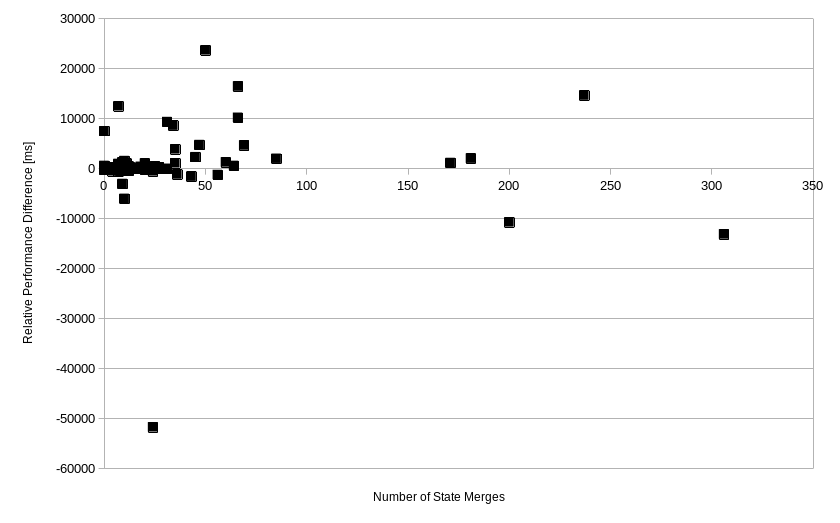
\includegraphics[width=\linewidth]{state-merges-vs-performance.png}
        \caption{
            Impact on the number of state merges on the performance,
            negative performance difference shows a speedup.
        }
        \label{fig:state-merges}
    \end{figure}

    Interestingly, the performance seems to improve about 3.3\% for programs
    with an absolute base verification time up to 0.5 seconds. With increasing verification
    time, the performance decreases, and for programs with a verification time greater
    than 10 seconds, we get a decrease of performance of nearly 25\%.
    
    This observation suggests for smaller programs where fewer joins are needed, the more complex symbolic
    states caused by joining is worth trading for the benefit of having fewer branches. For
    larger programs, the symbolic state may become overly complex up to a point that the advantage of
    fewer branches no longer pays off.

    \begin{figure}[H]
        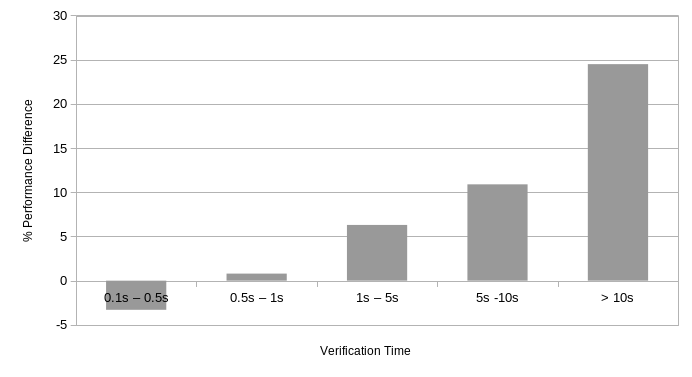
\includegraphics[width=\linewidth]{performance-change-vs-verification-time.png}
        \caption{
            Change in performance depending on absolute base verification time. Negative performance difference shows a speedup.
        }
        \label{fig:state-merges}
    \end{figure}

    \subsection{Complementary Benchmarks}

    As state merging currently empties caches instead of merging them, an option to disable the caches
    was added. Disabling caches results in a performance decrease of 1.9\%.

    Silicon additionally provides an option of enabling a more complete version of exhaling permissions,
    which must be used when joining is enabled. This is because joining may result in permissions of a 
    location being divided into multiple heap chunks. Benchmarks have shown that enabling more complete 
    exhale results in a performance increase of 2.9\%.

    \newpage
    \section{Future Work}

    

    \newpage
    \printbibliography
    
\end{document}